%results.tex%

\section{Results and Discussion} \label{results}
\subsection{Truncation considerations} \label{cutoffs}
As stated previously, the ``raw'' wave function features used to build machine-learning representations must be carefully selected. To illustrate this point, the TATR was used to model a carbon monoxide potential energy curve using the highest 150 amplitudes (by magnitude) and $M = 12$ training points as in Ref.~\citenum{Margraf2018}. 
Figure~\ref{fig:both_co_pes} shows that, when molecular symmetry is considered ($C_{2v}$, the largest Abelian subgroup of the full $C_{\infty v}$ point group), excellent regression results are produced using only 150 amplitudes. 

\begin{figure}
    \begin{subfigure}{.5\textwidth}
        \centering
        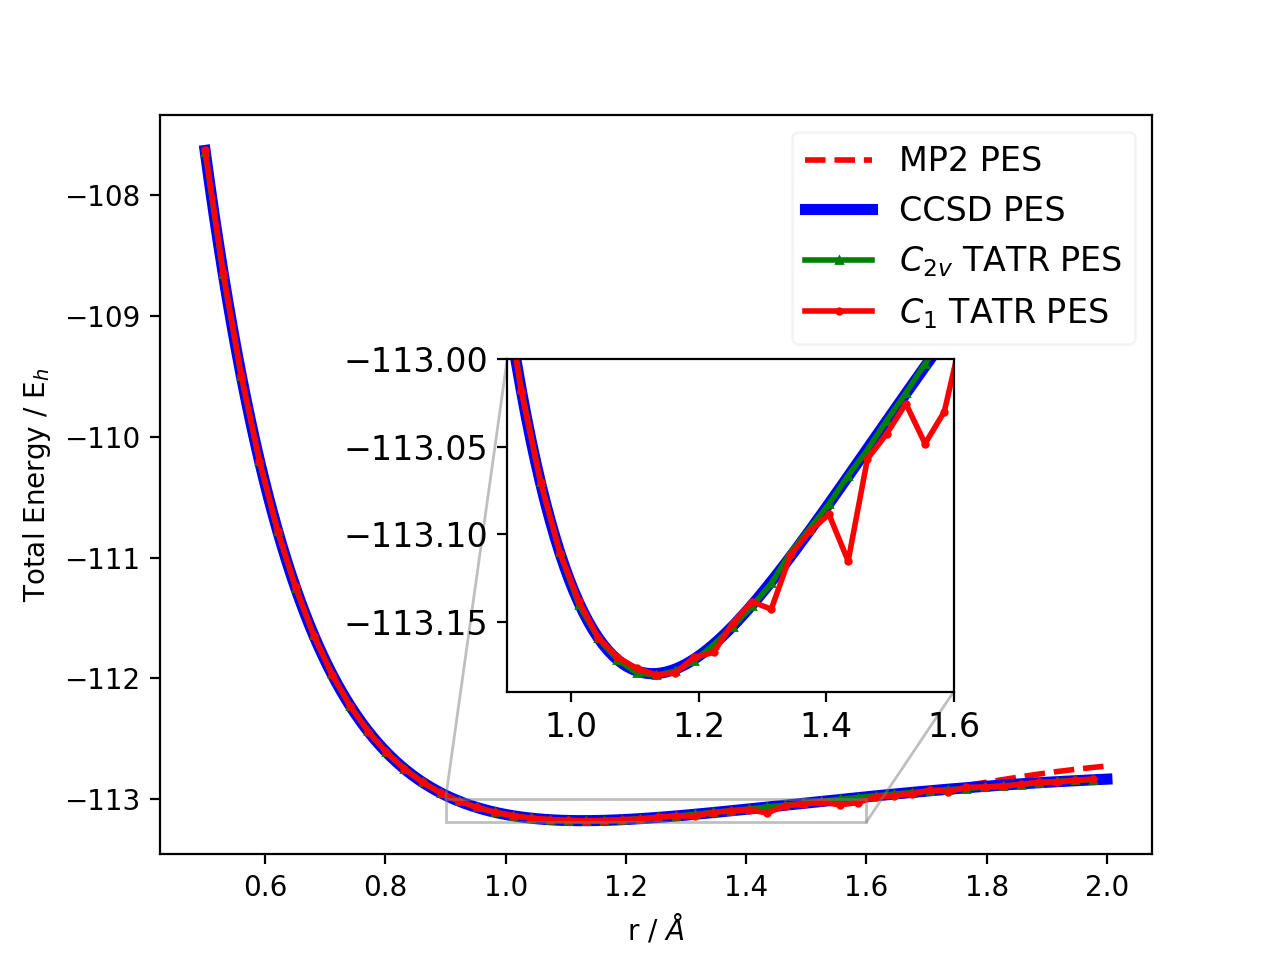
\includegraphics[scale=.5]{p2/figures/co_pes.png}
        \caption{}
        \label{fig:both_co_pes}
    \end{subfigure}
    \begin{subfigure}{.5\textwidth}
        \centering
        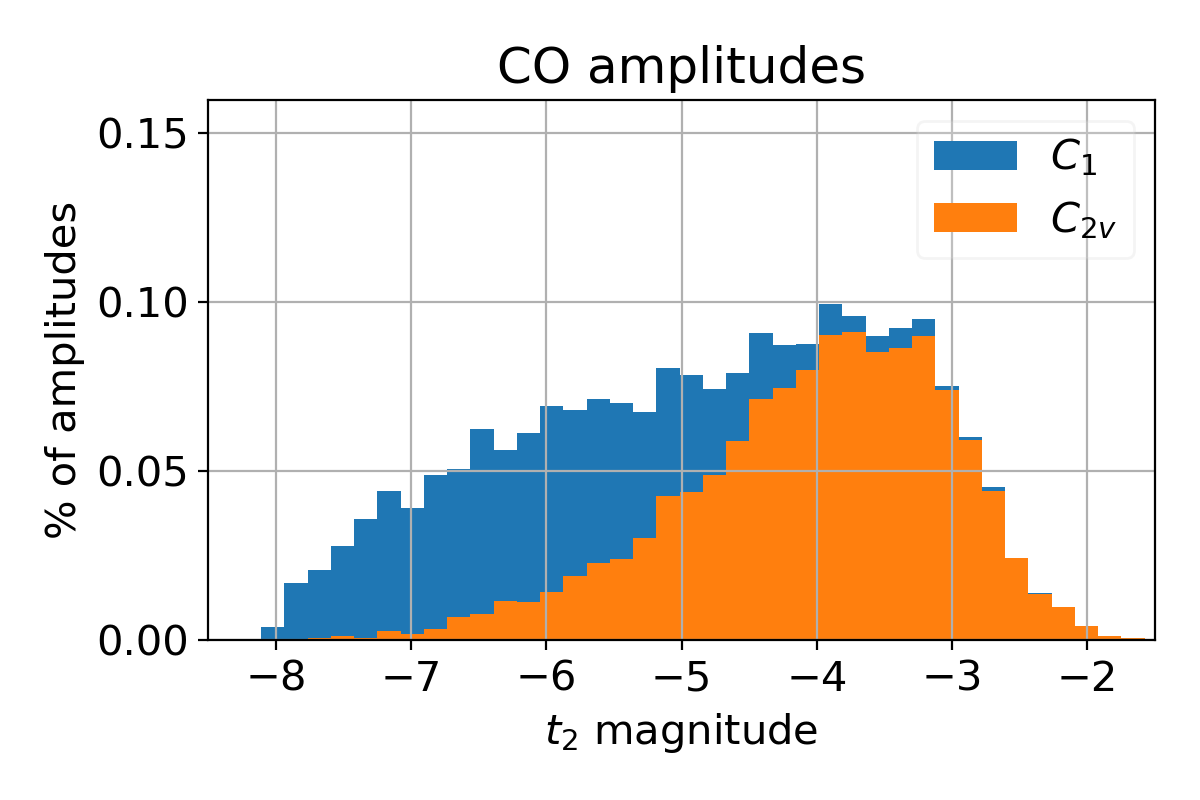
\includegraphics[scale=.5]{p2/figures/amp_dist.png}
        \caption{}
        \label{fig:amp_dist}
    \end{subfigure}
    \caption{(a) KRR for the carbon monoxide potential energy curve with and without molecular symmetry considered and (b) their respective amplitude distributions. TATR models used $M = 12$ training points. All amplitudes with magnitude $< 10^{-8}$ are set to 0.}
    \label{fig:CO_PES}
\end{figure}
However, to model the effect of decreased sparsity in the amplitudes on the representation, molecular symmetry was then dropped to $C_1$. When molecular symmetry is ignored, the number of ``significant'' ($>10^{-8}$) amplitudes greatly increases, as shown in Figure~\ref{fig:amp_dist}. 
In this case, taking only the highest 150 amplitudes no longer creates an effective representation of the wave function, resulting in poorer performance across the curve, also shown in Figure~\ref{fig:both_co_pes}.

This example shows a considerable disadvantage of the TATR, namely that the T2-amplitude tensor is in general very large 
(equal to the number of occupied orbitals squared times the number of virtual orbitals squared). It is, of course, in principle possible to build the TATR with an arbitrary number of amplitudes, as the size of the representation is independent of the number of amplitudes. However, using all amplitudes is not advisable, as a large number of negligible amplitudes would lead to large (but chemically meaningless) TATR values around zero. Meanwhile, without extensive testing, it is in general unclear how many amplitudes to retain for an effective representation. For this reason, a large number of amplitudes must in general be stored, at least for initial testing and hyperparameter optimization. Here cutoffs based on the amplitude magnitude may be employed, but this can still lead to significant storage requirements for larger molecules and basis sets. Figure~\ref{fig:CO_PES} also indicates that the TATR will likely not be applicable for larger systems that have no symmetry.
 
Storing the 1-RDM, on the other hand, only requires storing the number of basis functions squared floating point numbers. Furthermore, it is also known that the majority of significant elements in the MO-basis 1-RDM will be along the diagonal --- with some number of off-diagonal contributions. %is there a citation for this?
This gives a useful rule-of-thumb for how it could be truncated in extreme cases.
For the remainder of this manuscript, the TATR will be computed using the highest 150 amplitudes (by magnitude) computed in the highest symmetry available. The DTR will be computed using all 1-RDM elements.

\subsection{Energies} \label{energy}
In the spirit of comparing to previous results, the same diatomic potential energy curves from Ref.~\citenum{Margraf2018} were computed using the DTR. The prediction errors on the test set are shown in the Supporting Information, along with TATR results for comparison.
 Overall, DTR results do not vary significantly from the $C_{2v}$-symmetry TATR results for these systems; however, when molecular symmetry is not considered, a far greater number of amplitudes are required in the TATR to achieve the same accuracy.

To test the applicability of the DTR and TATR models to larger systems which may not benefit from molecular symmetry, geometries for water, methanol, (\textit{S})-methyloxirane, and (\textit{R})-methylthiirane near equilibrium were sampled randomly from a set of molecular dynamics (MD) trajectories and examined using both the TATR and DTR models.
Correlation energy data are presented in Figure~\ref{fig:small-E}. The prediction errors on the test set are plotted against the true CCSD correlation energy, ordered by increasing energy to evaluate how the model error varies with respect to the magnitude of the correlation energy.
Each point represents the prediction error of a single geometry along the MD trajectory.
As with the diatomics, most predictions lie well within the bounds of ``chemical accuracy'' (1.6mE$_h$). However, for the TATR, linear error centered around zero and which changes sign near the mean correlation energy value suggest that this model is biased towards the mean of the training set. 
While this still gives a rather agreeable mean-absolute-error across this particular test set, predictions for geometries far from the energetic minimum (i.e., sufficiently different from the training set) may not perform as admirably. This issue is explored further in section~\ref{alg_opt}.


\begin{figure}
    \begin{subfigure}{.5\textwidth}
        \centering
        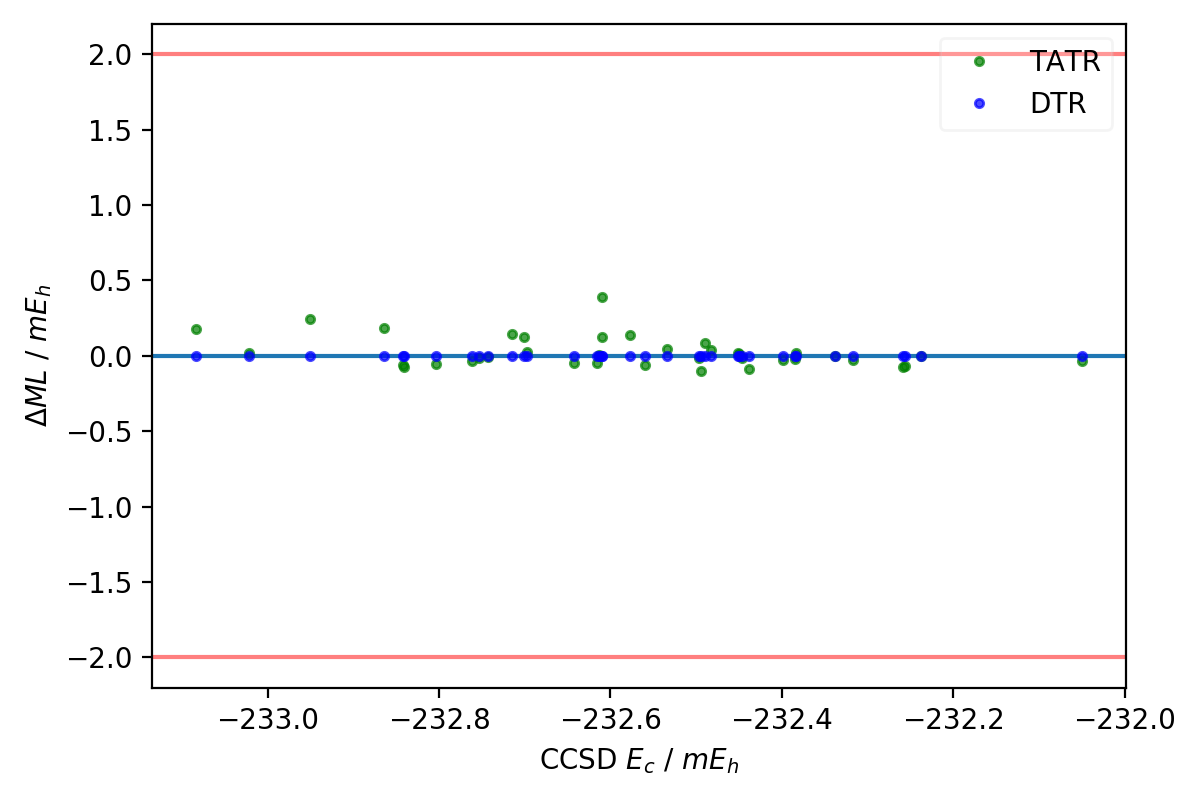
\includegraphics[scale=.55]{p2/figures/H2O_energy.png}
        \caption{}
        \label{fig:H2O}
    \end{subfigure}%
    \begin{subfigure}{.5\textwidth}
        \centering
        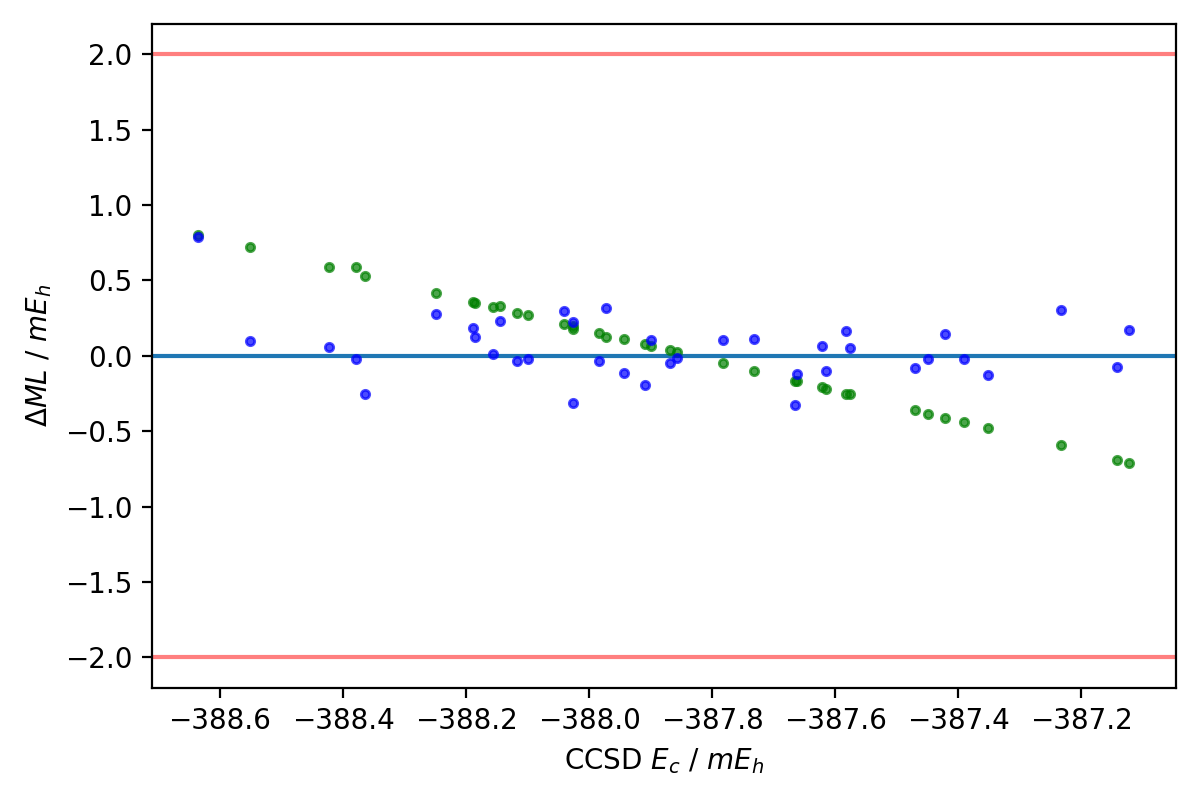
\includegraphics[scale=.55]{p2/figures/CH3OH_energy.png}
        \caption{}
        \label{fig:CH3OH}
    \end{subfigure}
    \begin{subfigure}{.5\textwidth}
        \centering
        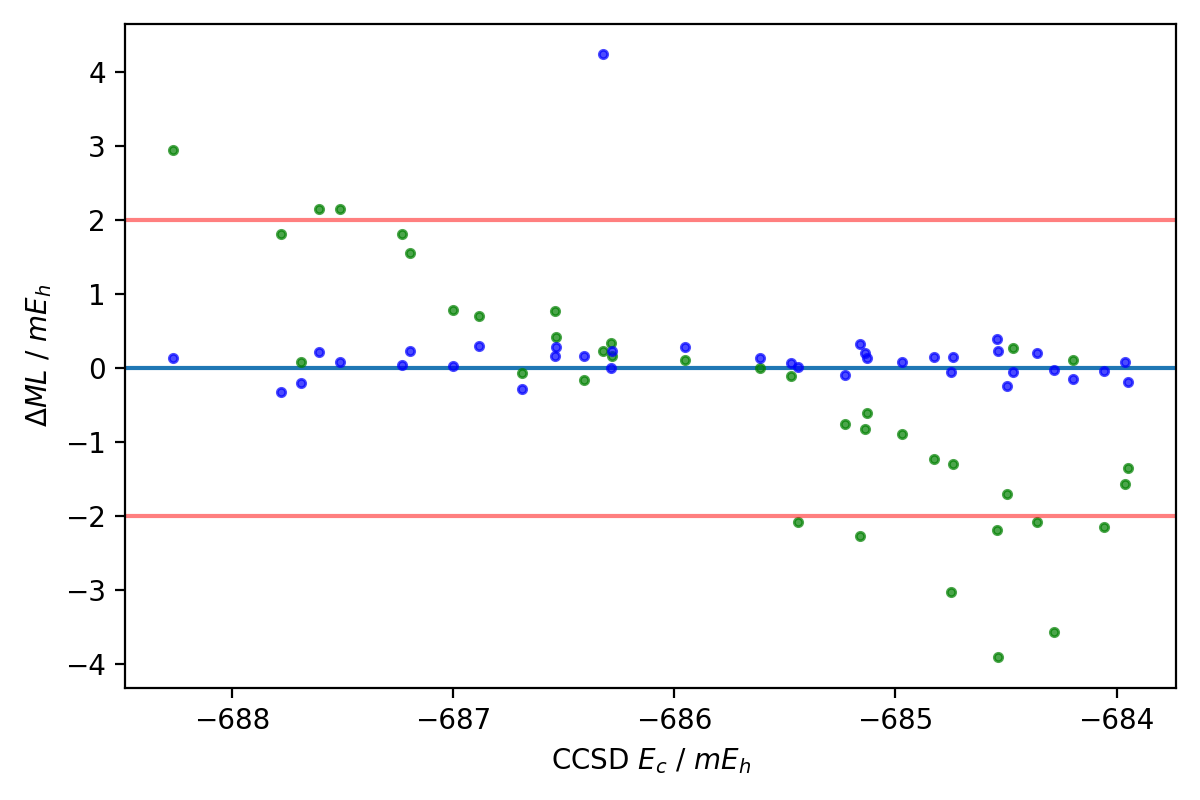
\includegraphics[scale=.55]{p2/figures/metox_energy.png}
        \caption{}
        \label{fig:METOX}
    \end{subfigure}%
    \begin{subfigure}{.5\textwidth}
        \centering
        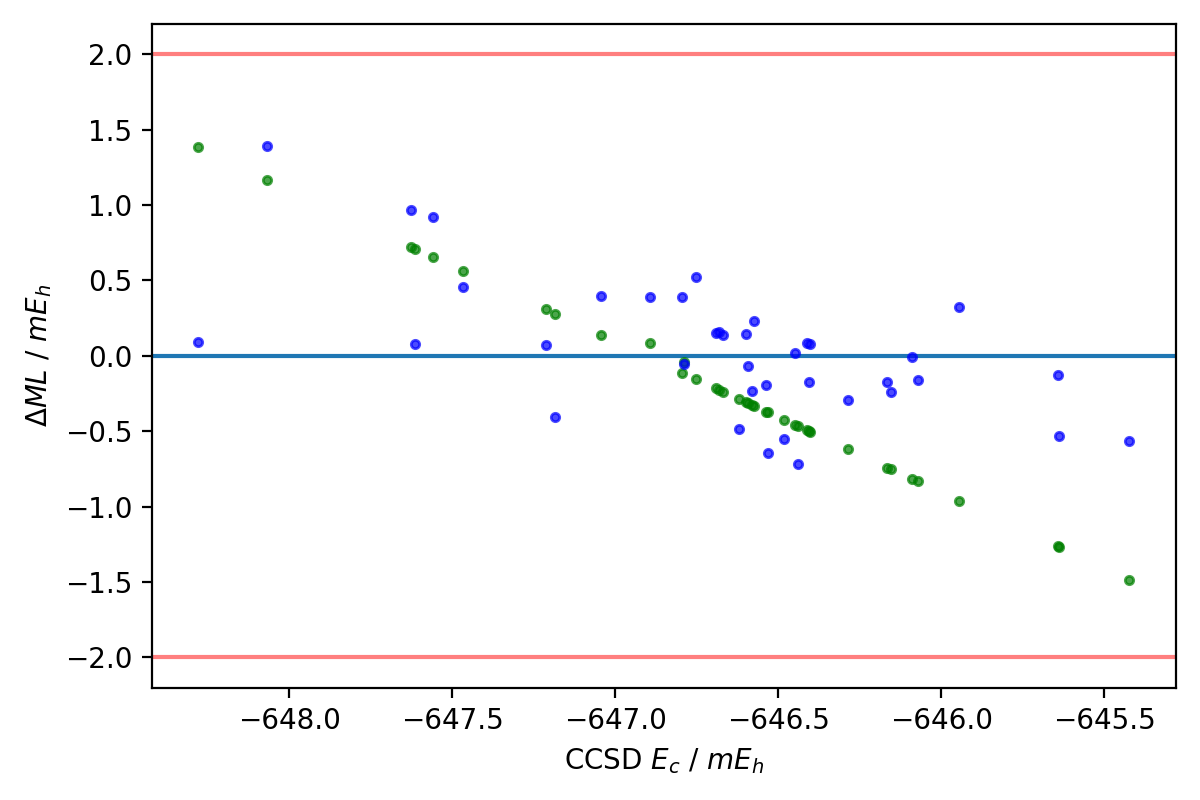
\includegraphics[scale=.55]{p2/figures/metthi_energy.png}
        \caption{}
        \label{fig:METTHI}
    \end{subfigure}
    \caption{DTR vs TATR errors in mE$_h$ for small molecule datasets: (a) H$_2$O, (b) CH$_3$OH, (c) ($\textit{S}$)-methyloxirane, and (d) ($\textit{R}$)-methylthiirane. Red lines indicate 2 mE$_h$.}
    \label{fig:small-E}
\end{figure}

A summary of energy results is shown for both the TATR and DTR methods in Figure~\ref{fig:E_sum}. 
The trained models reproduce the mean average correlation energy of the test set to within two milli-Hartree for every system considered. 
Furthermore, DTR errors are kept below 0.5 milli-Hartree for all systems except for CO and LiF. Inspection of their individual model performance (see the Supporting Information) reveals some difficulty in modeling the extreme ends of the curve (i.e. points far from the energetic average across the test set). These errors are also dominated by a relatively small number of outliers with increased errors. 
These examples also cover large ranges of correlation energies (100 and 60 milli-Hartree, respectively), which test both the regression capability and the validity of the underlying MP2 wave function used for the representation.  

\begin{figure}
    \centering
    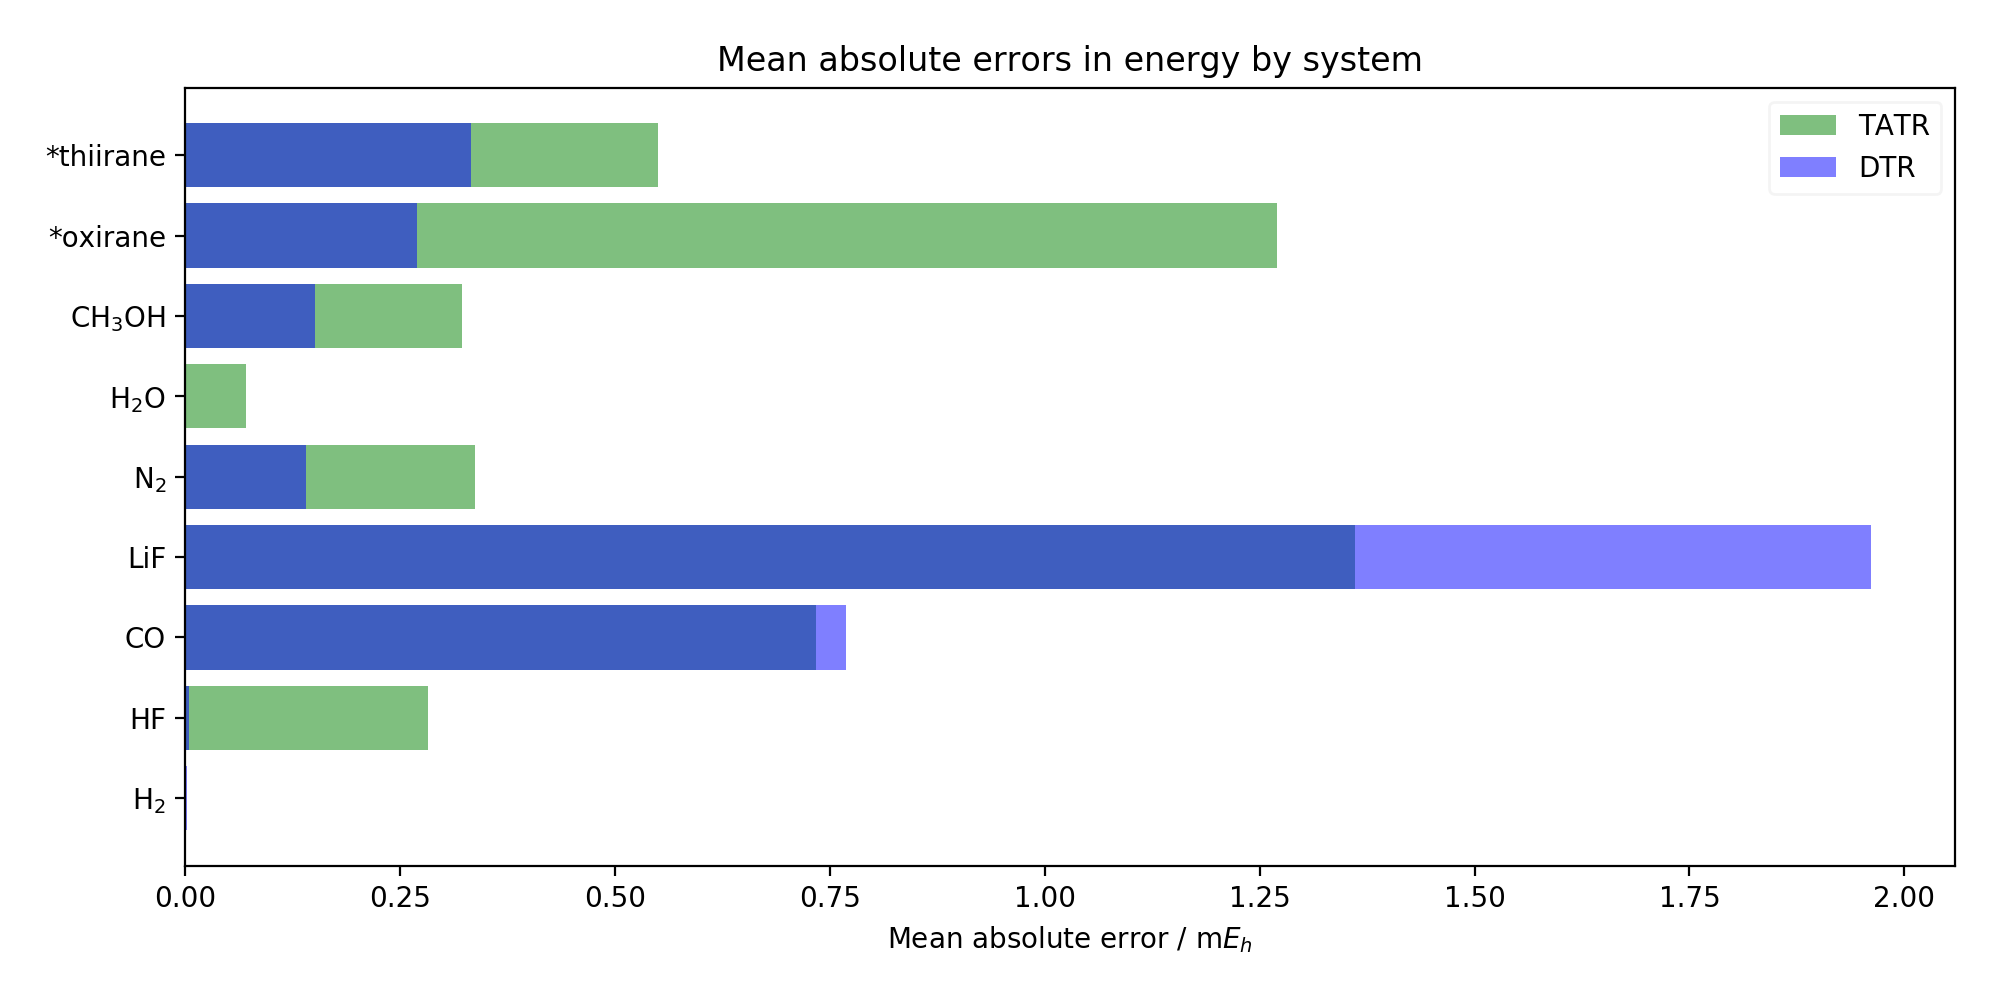
\includegraphics[angle=90, scale=.9]{p2/figures/E_err.png}
    \caption{DTR vs TATR errors in mE$_h$ for all datasets. (* = methyl)}
    \label{fig:E_sum}
\end{figure}

The energy data suggests that the improvements made by the DTR method result in greater accuracy in the molecular representation, in particular for larger molecules.
As shown in Ref.~\citenum{Margraf2018}, the electronic wave function can be well approximated using this relatively simple functional form when applied to energies. 
If this functional form is truly representative of the total wave function, rather than simply the parts which are important to the energy, then it should also be possible to compute molecular properties with a similar approach. 

\subsection{Dipole moments} \label{dip}

Several schemes for computing dipole moments were employed to emphasize the importance of Eq.~(\ref{eq:dipole}). 
Full density matrices $(D^{SCF} + D^{MP2})$ were used as raw features to build DTRs for learning total ($\mu^{T} = \mu^{e} + \mu^{nuc}$), electronic ($\mu^{e} = \mu^{SCF} + \mu^{CC}$), and correlated ($\mu^{CC}$) dipole moments.
MAEs (in Debye) for the machine-learned dipole moments, using each of the three possible target values, are given in Table~\ref{table:separability}.  
The MAEs for the MP2-level correlated dipole (relative to the CCSD result) for the same predicted sets are given for comparison.

\begin{table}[h]
\centering
\begin{tabular}{|c|c|c|c|c|}
    \hline
    Molecule & $\mu^{T}$ & $\mu^{e}$ & $\mu^{CC}$ & MP2 \\
    \hline
    H$_2$O & $1.5\times10^{-3}$ & $1.3\times10^{-3}$ & $1.8\times10^{-4}$ & $1.8\times10^{-2}$\\
    \hline
    CH$_3$OH & $3.8\times10^{-2}$ & $1.7\times10^{-1}$ & $2.1\times10^{-3}$ & $1.8\times10^{-2}$ \\
    \hline
    *oxirane & $1.0\times10^{-1}$ & $4.3\times10^{-1}$ & $5.7\times10^{-3}$ & $2.0\times10^{-2}$ \\
    \hline
    *thiirane & $5.4\times10^{-2}$ & $6.5\times10^{-1}$ & $7.3\times10^{-3}$ & $3.5\times10^{-2}$ \\
    \hline
\end{tabular}
\caption{Mean absolute errors (in Debye) relative to CCSD of four machine-learning datasets utilizing full, electronic, and correlated dipole moments as training targets. MP2 dipoles given for comparison. (* = methyl)} \label{table:separability}
\end{table}

As expected, minimizing the extrapolation necessary for the model reduces the error drastically. The error in the electronic component of the dipole moment in e.g. (\textit{S})-methyloxirane is reduced by an order of magnitude relative to using the full dipole moment. Furthermore, this error is also an order of magnitude lower than the MAE in the MP2 correlated dipole moments on the same predicted set. This is consistent with Ref.~\citenum{Margraf2018} where extremely accurate models for the \textit{correlation} energy were built. The same is clearly the case for the (correlated) dipole moment.

A summary of dipole results is shown for both the TATR and DTR methods in Figure~\ref{fig:D_sum}.
The same datasets as for correlation energy learning were considered, except for the homonuclear diatomics. As with the energy, the trained models reproduce the correlated dipole moment of the test sets to reasonable precision. 
Once again, the challenging cases of CO and LiF produce the maximum errors; however, it is encouraging that even here, errors for states near equilibrium (those modeled by molecular dynamics) are of milliDebye magnitude. % is there an abbreviation for milliDebye? 

Indeed, it has been shown (e.g. in Ref.~\citenum{Christensen2019}) that predicting dipole moments with ML is significantly more challenging than predicting energies. 
Still, our results support the notion that, as long as the reference wave function is sound, the molecular representation will ``correctly represent the physics of the problem''\cite{Margraf2018} as desired with a favorably small number of training points. While these results represent only a marginal improvement over the already sound MP2 approximation, they demonstrate that simple ML models effectively capture the characteristics of the wave function without the need for a complex functional form. They also show that this generalizes beyond the energy to molecular properties as well. 

\begin{figure}
    \centering
    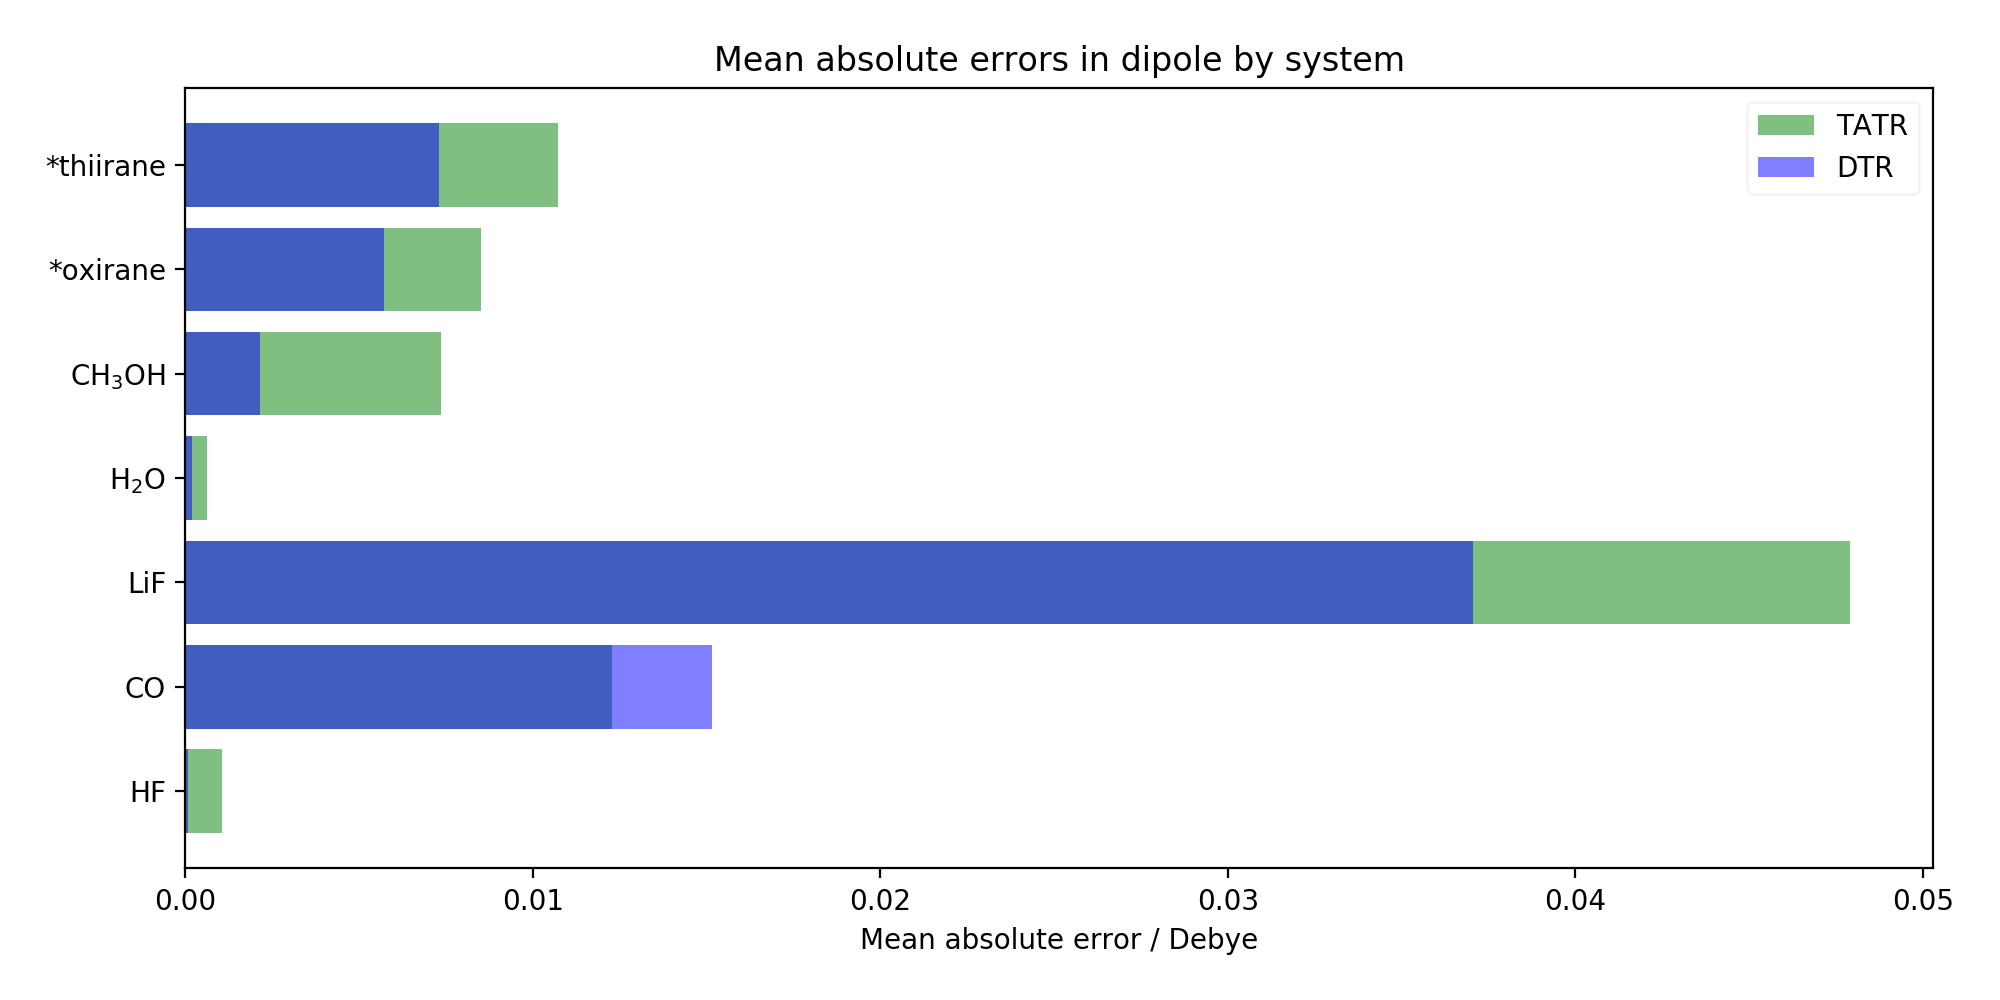
\includegraphics[angle=90, scale=.9]{p2/figures/D_err.png}
    \caption{DTR vs TATR errors in $milliDebye$ for all datasets. (* = methyl)}
    \label{fig:D_sum}
\end{figure}

\subsection{Extensions} \label{ext}
The present model can be used to solve a number of potential problems, mostly involving local PESs or dipole moment surfaces of small molecules which are amenable to MP2-level calculations (and a few CCSD training calculations). This is especially useful for generating accurate force field parameters\cite{Sauceda2019,Galvelis2019} and evaluating numerical gradients\cite{Schmitz2018a}. Furthermore, the DTR representation has been shown to provide high accuracy with very few training points, resulting in a highly data-efficient method. While this covers a significant space of applications, there are some areas which cannot currently be addressed, but could be well within reach of the proposed algorithm. 

\subsubsection{Transferability} 
The DTR-based machine-learning model as described above shows that a mapping from the MP2 1-RDM to CCSD electronic properties is feasible using a simple ML model. This allows avoiding the high-cost evaluation of the CC wave function for multiple geometries of the same molecule. However, if the method is to be generalized to different molecular systems (rather than just different geometries as we've shown here), additional modifications must be considered. Specifically, two (related) types of transferability are desirable: on one hand, a model can be transferable between different chemical compositions (i.e. trained on water and methane, applied to methanol)\cite{Welborn2018a}. 
On the other hand, a model can be transferable among different system sizes (i.e. trained on water clusters and applied to bulk water)\cite{Jung2020}.
 
The main impediment for both the TATR and the DTR to be transferable is the use of a molecular orbital basis, which is strongly system dependent. An obvious route towards more transferability would be to use the atomic orbital (AO) basis instead. In this representation, the molecular dependence of the representation would stem only from the identity of the basis functions placed on each atom. While this still precludes transferability between different elements, this is not very problematic in practice, as one can always train on the elements of interest.
Regarding transferability to different sizes, this essentially boils down to the requirement that the ML model be size extensive. The lack of extensivity is a common weakness of ML models that use global representations such as the DTR or TATR. As recently discussed by Jung et al., global KRR models can be made size extensive, however, if the Kernel function is properly normalized\cite{Jung2020}. While that study focused on representations of the molecular geometry, it would certainly be worthwhile exploring how extensive models based on wave function representations would perform.

Finally, a theoretical consideration can also be made with respect to transferability. As mentioned above, one-electron properties can be described by the general form of Eq.~(\ref{eq:prop}). Comparing this to the KRR equations (see Eq.~(\ref{eq:krr})), and considering that the kernel only includes information from the 1-RDM, it can be inferred that the coefficients $\mathbf{\alpha}$ are modelling the contributions arising from the property integrals, $\bra{p}\Omega\ket{q}$.
In the present model, however, the coefficients are also doing the job of mapping the low-level (MP2) representation onto the high-level (CCSD) target function. To truly separate the molecule-specific terms from the correlation contributions, the property integrals (in a transferable basis, such as the AO basis) should thus also be included in the representation of the molecule. 
Modifications such as using product kernels to fold in the contribution from the integrals can be explored to correct this shortcoming.

\subsubsection{Additional properties}
Properties beyond dipole moments are also accessible, but not without modifications. While first-order one-electron properties are available through Eq.~(\ref{eq:prop}), considerations of both the one- and two-electron densities is generally necessary for two-electron properties. 
Fortunately, we have seen that the 1-RDM suffices to predict at least one property which depends on both the 1- and 2-RDM, namely the energy. This may be related to the special formulation of 1- and 2-RDMs in MP2, as discussed above. It could also be a particular property of the ground-state energy which, according to the Hohenberg and Kohn theorem\cite{Hohenberg1964}, formally only depends on the ground state density (and thus the 1-RDM).
However, this is not generally the case, for example in CC response theory. Higher-order properties in CC response depend on both the 1- and 2-RDMs.
%, built from the t- and $\lambda$-amplitudes and their perturbed counterparts.  
Extensions to include both density matrices could be made, as with a singles-and-doubles TATR, though considerable truncation procedures would need to be implemented in order to keep storage costs reasonable across realistic datasets. 

Alternatively, second-order properties which depend only on one-electron operators, such as polarizabilities and chiroptical response, could also be considered using a reformulated CC linear response (CC-LR).  
It can be shown that, similarly to first-order properties, second-order response properties of this type can be expressed using the 1-RDM only. This is achieved by computing the first-order perturbed left-hand wave function parameters, $\lambda^{(1)}$.
Using these, second-order properties are computed in CC-LR as 
products of property integrals with \textit{perturbed} one-electron reduced density matrices\cite{Crawford2019}. 
Contributions from one operator are folded into the 1-RDM, and contributions from the other are described by the property integrals. In the context of the DTR, the density representation would now require only this perturbed 1-RDM with no additional changes. Contributions from property integrals may also be included in the representation, perhaps through the same sort of generalizations made to allow for transferability. In this fashion, many linear response properties could be made accessible. 

We will acknowledge one final potential oversight in property predictions done in the preceding manner:
a new model must still be trained for each property. 
To allow for a ``one-shot'' model prediction of arbitrary properties, the wave function itself (or some usable representation thereof) must be learned. 
This has recently been explored by Sch\"{u}tt and coworkers\cite{Schutt2019}, 
which has proved some efficacy of this strategy. 
Additional work on the usability of such representations will be considered while algorithms to learn the representation itself are formulated.
In practice, however, once the ground state equations (e.g. the amplitudes in CC theory) are solved, it is not necessary to recompute them for additional properties. Instead, the (linear) response function can be evaluated at this time for a multitude of properties.
Because of this, we suggest that many properties are computed and stored in a database when proposing and gathering reference or training data for ML algorithms, such as those provided in QCArchive\cite{Smith2020a}.

\subsubsection{ML algorithm optimization} \label{alg_opt}
Aside from coding additional physics into the representation and returning more varied properties, the ML workflow itself may also be optimized to be more data-efficient, accurate, and precise across varied molecular representations. To further evaluate model performance and perhaps diagnose potential problems, learning curves were generated for every system considered. These curves plot the error in the test (the ``validation curve'') and training (``training curve'') sets with respect to the number of training points used, with values ranging from two to one-hundred training points. The validation curve exposes the limitations of the current model by testing whether the model can be made more accurate using more training points. The training curve, on the other hand, describes how well the model is adhering to the training set, and so reveals problems of under- or over-training. Together, the curves indicate the practical limitations of the model's accuracy and use of data, suggesting an irreducible error that can only be addressed by changing the model or the representation itself. Learning curves for all systems considered are available in the Supporting Information.

The data discussed within the manuscript so far (excluding section ~\ref{cutoffs}) has been collected using $M = 20$ training points, which result in the data points at that value in every validation curve.
In a log-log plot, the validation curve should be linear such that an increase in the number of training points results in a commensurate decrease in error. 
This is well exhibited by, e.g., the validation curve for predicting the correlation energy for ($\textit{S}$)-methyloxirane, Figure~\ref{fig:metox_E_learn}. 
Generally, the DTR validation curve starts lower than the TATR. The DTR model also tends to benefit more from additional training points in the two- to fifty-point range. 
It is important to note that the most significant outliers to this trend are the dipole moment models for ($\textit{S}$)-methyloxirane and ($\textit{R}$)-methylthiirane (see SI), the largest molecules considered and undoubtedly the most complex electronic environments. These systems benefit from larger training sets and are more prone to fortuitously low errors with small training sets, requiring a careful analysis of the validation curve before deciding on an optimal training set size.
This is, of course, subject to the constraint that the training points are still taken from near-equilibrium values. Improving the quality of the training set by including more distinct electronic states away from equilibrium may improve performance.

\begin{figure}
    \centering
    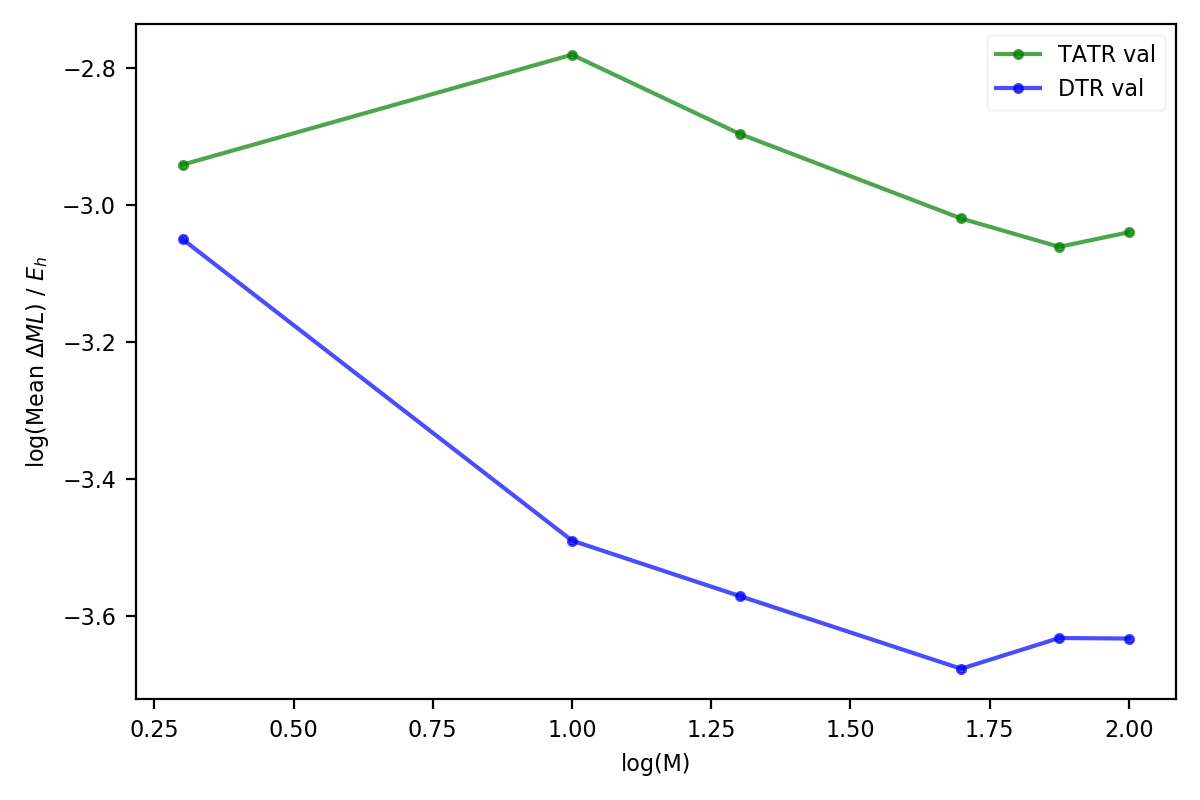
\includegraphics[scale=.75]{p2/figures/metox_log_learn.png}
    \caption{DTR and TATR validation curves for ($\textit{S}$)-methyloxirane correlation energy.}
    \label{fig:metox_E_learn}
\end{figure}

In considering the training curves (see SI), it is revealed that the TATR suffers from increased training error as compared to the DTR, referred to as \textit{bias}. 
Bias (sometimes referred to as \textit{inductive bias})\cite{Rasmussen2006} refers to error arising from simplifying assumptions made in the model: in this case, the small number of amplitudes retained is the most obvious source of additional bias. 
As this bias causes high training errors, it suggests that the TATR model is not fitting the training data as well as the DTR. This is likely the cause of the linear errors discussed in setion~\ref{energy}, as the model is simply learning toward the mean of the training set, rather than properly reproducing each point. 
These errors can be reduced by improving the model, e.g. by including more amplitudes in the TATR or by the DTR modifications described above.
Additional features or a reformulation of the representation may also be explored using automated model-selection routines, such as those employed in Ref.~\citenum{Chen2020}. These routines would, in theory, result in a more complex model accessing a higher dimensional feature space, so the challenges of extension become ensuring that this model still fits the training data (does not under-train as a result of bias) and generalizes to unseen data (does not over-train as a result of variance) when compared to a simpler approach.

